\documentclass[11pt,a4paper]{article}

\usepackage[a4paper,margin=22mm]{geometry}
\usepackage{fontspec}
\usepackage{microtype}
\usepackage{amsmath}
\usepackage{amssymb}
\usepackage{booktabs}
\usepackage{array}
\usepackage{tabularx}
\usepackage{siunitx}
\usepackage{xcolor}
\usepackage{tikz}
\usepackage{pgfplots}
\usepackage[most]{tcolorbox}
\usepackage{hyperref}
\usepackage{enumitem}
\usepackage{titlesec}
\usepackage{fancyhdr}

\pgfplotsset{compat=1.18}
\usetikzlibrary{arrows.meta,positioning,calc,shapes.geometric,patterns,fit,decorations.pathreplacing}

\setmainfont{Latin Modern Roman}
\setsansfont{Latin Modern Sans}
\setmonofont{Latin Modern Mono}

\definecolor{Ink}{HTML}{172033}
\definecolor{Muted}{HTML}{657083}
\definecolor{Blue}{HTML}{1D6CDF}
\definecolor{Teal}{HTML}{0E9F9A}
\definecolor{Orange}{HTML}{D97706}
\definecolor{Red}{HTML}{C2410C}
\definecolor{Green}{HTML}{15803D}
\definecolor{Panel}{HTML}{F5F7FB}
\definecolor{Line}{HTML}{D7DEE8}
\definecolor{DarkPanel}{HTML}{101827}

\hypersetup{
  colorlinks=true,
  linkcolor=Blue,
  urlcolor=Blue,
  citecolor=Blue,
  pdftitle={Deterministic Sobol European Option Pricing},
  pdfauthor={European Option Engine}
}

\pagestyle{fancy}
\fancyhf{}
\lhead{\textcolor{Muted}{Deterministic Sobol European Option Pricing}}
\rhead{\textcolor{Muted}{\thepage}}
\renewcommand{\headrulewidth}{0.3pt}
\renewcommand{\headrule}{\hbox to\headwidth{\color{Line}\leaders\hrule height \headrulewidth\hfill}}

\titleformat{\section}
  {\Large\sffamily\bfseries\color{Ink}}
  {\thesection}{0.6em}{}
\titleformat{\subsection}
  {\large\sffamily\bfseries\color{Ink}}
  {\thesubsection}{0.6em}{}

\setlist[itemize]{leftmargin=*,itemsep=2pt,topsep=3pt}
\setlength{\parindent}{0pt}
\setlength{\parskip}{7pt}
\setlength{\headheight}{24pt}
\renewcommand{\arraystretch}{1.18}

\newtcolorbox{keybox}[1]{
  enhanced,
  colback=Panel,
  colframe=Blue!45,
  title=#1,
  fonttitle=\sffamily\bfseries,
  coltitle=Ink,
  boxrule=0.7pt,
  arc=2mm,
  left=3mm,
  right=3mm,
  top=2mm,
  bottom=2mm
}

\newtcolorbox{warnbox}[1]{
  enhanced,
  colback=Orange!7,
  colframe=Orange!65,
  title=#1,
  fonttitle=\sffamily\bfseries,
  coltitle=Ink,
  boxrule=0.7pt,
  arc=2mm,
  left=3mm,
  right=3mm,
  top=2mm,
  bottom=2mm
}

\newcommand{\code}[1]{\texttt{#1}}
\newcommand{\normalcdf}{\Phi}

\begin{document}

\begin{titlepage}
\begin{tikzpicture}[remember picture,overlay]
  \fill[DarkPanel] (current page.south west) rectangle (current page.north east);
  \fill[Blue!70!black] (current page.north west) rectangle ($(current page.north east)+(0,-34mm)$);
  \draw[Blue!45,line width=0.6pt] ($(current page.south west)+(18mm,18mm)$) rectangle ($(current page.north east)+(-18mm,-18mm)$);
  \foreach \x in {0,1,...,15} {
    \draw[white!6,line width=0.25pt] ($(current page.south west)+(\x*15mm,0)$) -- ($(current page.north west)+(\x*15mm,0)$);
  }
  \foreach \y in {0,1,...,22} {
    \draw[white!5,line width=0.25pt] ($(current page.south west)+(0,\y*13mm)$) -- ($(current page.south east)+(0,\y*13mm)$);
  }
\end{tikzpicture}

\vspace*{18mm}
{\sffamily\bfseries\color{white}\fontsize{32}{38}\selectfont
Deterministic Sobol\\European Option Pricing\par}
\vspace{5mm}
{\sffamily\color{white!78}\fontsize{15}{20}\selectfont
A white paper on the fused Sobol, Gaussian transform, exponential payoff, and reduction path\par}

\vfill
\begin{tikzpicture}
  \node[
    draw=Teal!70,
    fill=DarkPanel,
    rounded corners=2mm,
    line width=0.8pt,
    text width=0.70\textwidth,
    minimum height=31mm,
    inner sep=6mm,
    align=left
  ] {
    {\color{white}\sffamily\bfseries Executive summary}\\[2mm]
    {\color{white!82}
    The engine uses the deterministic order of a dimension-1 Sobol sequence to
    avoid general-purpose random-number post-processing. For most lanes, it does
    not store Gaussian values and does not call a runtime exponential. Instead,
    it evaluates a small local payoff polynomial whose coefficients are prepared
    once for the contract.}
  };
\end{tikzpicture}

\vfill
{\color{white!65}\sffamily Private technical note. Generated from the current AVX-512 pricing prototype.}
\end{titlepage}

\tableofcontents
\newpage

\section{The Pricing Problem}

A European option has a payoff at one future time. In the Black--Scholes model,
the terminal stock price is
\[
  S_T = S_0 \exp\left((r - \tfrac{1}{2}\sigma^2)T + \sigma\sqrt{T}\,Z\right),
\]
where \(Z\) is a standard normal random variable. The discounted payoff is
\[
  C = e^{-rT}\max(S_T-K,0)
  \quad\text{for a call,}
\]
and
\[
  P = e^{-rT}\max(K-S_T,0)
  \quad\text{for a put.}
\]

In a Monte Carlo or quasi-Monte Carlo engine, the normal variable \(Z\) usually
comes from a uniform number \(u\in[0,1]\) through the inverse normal CDF:
\[
  Z = \normalcdf^{-1}(u).
\]

\begin{keybox}{What the engine changes}
The usual calculation creates or streams intermediate values:
Sobol uniforms, Gaussian values, exponentials, payoffs, and finally a sum.
The new engine collapses most of those stages. In the steady-state path, a Sobol
lane is transformed directly into a discounted payoff contribution.
\end{keybox}

\section{The Conventional Path}

The conventional path is easy to understand but expensive:

\begin{center}
\begin{tikzpicture}[
  node distance=4mm,
  proc/.style={draw=Line,fill=Panel,rounded corners=2mm,minimum width=24mm,minimum height=10mm,align=center,font=\sffamily},
  arr/.style={-Latex,thick,draw=Blue}
]
  \node[proc] (sobol) {Sobol\\uniform \(u\)};
  \node[proc,right=of sobol] (gauss) {Inverse CDF\\\(Z=\Phi^{-1}(u)\)};
  \node[proc,right=of gauss] (exp) {Stock price\\\(S_T=S_0e^{\mu+\alpha Z}\)};
  \node[proc,right=of exp] (payoff) {Payoff\\and discount};
  \node[proc,right=of payoff] (sum) {Reduction\\price};
  \draw[arr] (sobol) -- (gauss);
  \draw[arr] (gauss) -- (exp);
  \draw[arr] (exp) -- (payoff);
  \draw[arr] (payoff) -- (sum);
\end{tikzpicture}
\end{center}

This path is robust and general. It is also doing work that is not always needed
for a fixed, deterministic Sobol layout:

\begin{itemize}
  \item The inverse CDF is a nonlinear function with expensive tail handling.
  \item The exponential is another nonlinear function.
  \item Intermediate arrays create memory traffic.
  \item General-purpose libraries must handle arbitrary input order and
        arbitrary distributions.
\end{itemize}

\section{The Key Observation: Deterministic Sobol Slots}

Sobol points are not random in the usual sense. They follow a deterministic
digital-net pattern. The current engine uses dimension 1 and a public block size
of \(8192\) samples. Internally, each public block is processed as two
\(4096\)-sample chunks, and each hot loop step handles two AVX-512 registers:

\[
  2 \times 16 = 32 \text{ float values per store-pair slot.}
\]

For all steady-state chunks after the prefix, the relevant ranges repeat in a
known order. That makes the following possible:

\begin{center}
\begin{tikzpicture}[x=0.9cm,y=0.75cm,font=\sffamily\small]
  \draw[->,thick] (0,0) -- (13.2,0) node[right] {slot order};
  \foreach \i/\c in {0/Blue,1/Teal,2/Blue,3/Orange,4/Blue,5/Teal,6/Blue,7/Red,8/Blue,9/Teal,10/Blue,11/Orange} {
    \fill[\c!22] (\i,0.15) rectangle ++(0.8,1.0);
    \draw[\c!75!black] (\i,0.15) rectangle ++(0.8,1.0);
  }
  \node[align=left,anchor=west] at (0,1.6) {The range/sign class of each slot is known before runtime.};
  \node[anchor=west,text=Blue!80!black] at (0,-0.55) {normal};
  \node[anchor=west,text=Orange!85!black] at (2.0,-0.55) {hard};
  \node[anchor=west,text=Red!85!black] at (3.8,-0.55) {tail};
  \draw[decorate,decoration={brace,amplitude=5pt},thick,Muted] (0,1.25) -- (12.8,1.25)
    node[midway,yshift=13pt,text=Muted] {one repeated schedule};
\end{tikzpicture}
\end{center}

The important point is not that the sequence is simple. It is that the engine
knows where it is in the sequence. That lets the implementation avoid asking,
for every lane, ``which range am I in?''.

\section{Mantissa Injection}

A 32-bit floating-point value in \([1,2)\) has exponent bits fixed to
\(127\), and the mantissa carries the fractional position. The engine takes the
top bits of the Sobol integer and injects them into a float with exponent 1:

\[
  x = 1 + u,\quad x\in[1,2).
\]

In assembly this is the familiar pattern:

\[
  \text{shift Sobol integer} \rightarrow
  \text{OR with }0x3F800000.
\]

That is cheaper than fully normalizing to \(u\in[0,1]\), and it gives the local
polynomial a stable input coordinate.

\begin{center}
\begin{tikzpicture}[font=\sffamily\small]
  \draw[thick] (0,0) rectangle (12,1);
  \fill[Blue!18] (0,0) rectangle (2.2,1);
  \fill[Teal!18] (2.2,0) rectangle (12,1);
  \draw (2.2,0) -- (2.2,1);
  \node at (1.1,0.5) {exponent};
  \node at (7.1,0.5) {Sobol mantissa bits};
  \node[anchor=west] at (0,-0.55) {\(0x3F800000\)};
  \node[anchor=east] at (12,-0.55) {\(x=1+u\)};
  \draw[-Latex,thick,Blue] (6,1.3) -- (6,1.02);
  \node[align=center] at (6,1.75) {integer Sobol state\\becomes a float coordinate};
\end{tikzpicture}
\end{center}

\section{From Gaussian Transform to Direct Payoff}

The earlier Gaussian path used scheduled linear coefficients for normal slots:
\[
  Z(x) \approx g_0 + g_1x.
\]

The European payoff needs
\[
  \exp(\mu + \alpha Z(x)),\quad
  \alpha = \sigma\sqrt{T},\quad
  \mu=(r-\tfrac12\sigma^2)T.
\]

For a call option, after discounting and factoring out constants:
\[
  \text{payoff}(x) =
  \max\left(A\exp(\alpha(g_0+g_1x)) - B,\;0\right),
\]
where
\[
  A=e^{-rT}S_0e^{\mu},\qquad B=e^{-rT}K.
\]

For a put, the same shape is used with signed coefficients:
\[
  \text{payoff}(x) =
  \max\left(-A\exp(\alpha(g_0+g_1x)) + B,\;0\right).
\]

Instead of evaluating the exponential in the hot loop, contract setup composes
the already chosen exponential polynomial with the Gaussian affine model. Let
\[
  E(t) \approx e^t
\]
be the baked polynomial used by the fused kernel, and let \(m\) be the
deterministic center of this Sobol slot. Define
\[
  t_m = \alpha(g_0+g_1m),\qquad s=\alpha g_1.
\]

For a call away from the strike kink, the discounted local payoff is
\[
  f(x)=A\,E(t_m+s(x-m))-B.
\]
The quadratic coefficients follow directly from derivatives of \(E\):
\[
  p_0=A\,E(t_m)-B,
\]
\[
  p_1=A\,E'(t_m)\,s,
\]
\[
  p_2=\tfrac12 A\,E''(t_m)\,s^2.
\]

For a put, the same formulas are used with the signed scale and offset:
\[
  f(x)=-A\,E(t_m+s(x-m))+B.
\]
If the small local cell crosses the payoff boundary, setup handles that slot as
a kink cell using the same baked polynomial; it still avoids per-slot library
exponential calls.

In both cases, the hot loop only needs
\[
  f(x) \approx p_0 + p_1(x-m) + p_2(x-m)^2.
\]

\begin{keybox}{The core hot-loop idea}
For normal slots, the expensive composition
\[
  u \rightarrow Z \rightarrow \exp(\mu+\alpha Z) \rightarrow \text{payoff}
\]
is replaced by a local polynomial directly in the mantissa-injected Sobol
coordinate \(x=1+u\).
\end{keybox}

\section{Numerical Example}

Use the standard benchmark contract:
\[
  S_0=100,\quad K=100,\quad r=0.05,\quad \sigma=0.2,\quad T=1.
\]

Then
\[
  \mu = (0.05 - 0.5\cdot0.2^2)\cdot1 = 0.03,
\]
\[
  \alpha = 0.2\sqrt{1}=0.2,
\]
\[
  e^{-rT}=e^{-0.05}\approx0.951229.
\]

For a call, the setup scale is
\[
  A=e^{-rT}S_0e^\mu
   \approx 0.951229\cdot100\cdot e^{0.03}
   \approx 98.0199,
\]
and
\[
  B=e^{-rT}K \approx95.1229.
\]

Suppose a deterministic slot has local center
\[
  m=1.625.
\]
If its Gaussian affine model for this slot is
\[
  Z(x)\approx -0.80 + 0.50x,
\]
then at the center:
\[
  Z(m)\approx -0.80 + 0.50\cdot1.625 = 0.0125.
\]
The scaled exponent at the center is
\[
  t_m=\alpha Z(m)=0.2\cdot0.0125=0.0025.
\]
The call payoff model at the center is
\[
  \max(98.0199\cdot E(0.0025) - 95.1229,0)
  \approx 3.142.
\]
The first derivative coefficient is approximately
\[
  p_1 \approx 98.0199\cdot E'(0.0025)\cdot(0.2\cdot0.50),
\]
and the curvature coefficient is approximately
\[
  p_2 \approx \tfrac12\cdot98.0199\cdot E''(0.0025)\cdot(0.2\cdot0.50)^2.
\]

The real engine computes these coefficients for every deterministic slot at
contract setup by algebraically composing the polynomial pieces. The assembly
then processes each lane with a subtract, two fused multiply-add instructions,
a max against zero, and an accumulation.

\section{Visualizing the Local Approximation}

\begin{center}
\begin{tikzpicture}
\begin{axis}[
  width=0.86\textwidth,
  height=58mm,
  xlabel={local coordinate \(x-m\)},
  ylabel={discounted payoff},
  grid=both,
  grid style={Line!65},
  axis line style={Muted},
  tick style={Muted},
  legend style={draw=none,fill=none,at={(0.03,0.97)},anchor=north west},
  xmin=-0.00014,xmax=0.00014,
  ymin=3.10,ymax=3.19,
  scaled x ticks=false,
  xtick={-0.00012,-0.00006,0,0.00006,0.00012},
  xticklabels={$-1.2{\cdot}10^{-4}$,$-6{\cdot}10^{-5}$,$0$,$6{\cdot}10^{-5}$,$1.2{\cdot}10^{-4}$},
  x tick label style={font=\scriptsize}
]
\addplot[domain=-0.00013:0.00013,samples=120,Blue,very thick]
  {3.142 + 310*x + 1750*x*x};
\addlegendentry{local quadratic}
\addplot[domain=-0.00013:0.00013,samples=120,Orange,dashed,thick]
  {3.142 + 310*x + 1760*x*x + 200000*x*x*x};
\addlegendentry{true smooth payoff, illustrative}
\addplot[only marks,mark=*,mark size=1.9pt,Teal]
  coordinates {(-0.000122,3.1042) (0,3.142) (0.000122,3.1801)};
\addlegendentry{derivative anchor points}
\end{axis}
\end{tikzpicture}
\end{center}

The figure is illustrative, but it captures the engineering reason the method
works: each local interval is tiny. The quadratic is not trying to approximate
the whole payoff function. It only approximates the payoff over the small
neighborhood that a deterministic Sobol slot can visit.

\section{Where the First Block and Tails Differ}

The first Sobol prefix is special. It contains the origin and early points whose
range schedule does not match the steady-state repeated schedule. The engine
therefore patches known first-block vectors.

The extreme tail slots are also special. The inverse normal CDF changes quickly
near 0 and 1. For those lanes, the current implementation keeps a safer
Gaussian/tail path instead of forcing everything through the direct quadratic
normal-slot path.

\begin{warnbox}{Why one-block runs look weak}
At one block, the special prefix and setup overhead are a large part of the
entire timed run. At many blocks, the steady-state path dominates and the fixed
cost is amortized.
\end{warnbox}

\section{Benchmark Snapshot}

The following results were run on an AWS EC2 instance. The exact instance type
and CPU model were not captured in the snapshot.

\begin{center}
\small
\begin{tabular}{llrrrrrr}
\toprule
Type & Blocks & Samples & SDK ns/value & MKL full & MKL Sobol & vs full & vs Sobol\\
\midrule
call & 1    & 8,192      & 10.023682 & 5.451050 & 0.109009 & 0.54x & 0.01x\\
put  & 1    & 8,192      &  9.969727 & 5.200562 & 0.109131 & 0.52x & 0.01x\\
call & 128  & 1,048,576  &  0.233498 & 5.257521 & 0.188629 & 22.52x & 0.81x\\
put  & 128  & 1,048,576  &  0.227925 & 5.016124 & 0.187053 & 22.01x & 0.82x\\
call & 1221 & 10,002,432 &  0.159627 & 5.331564 & 0.201620 & 33.40x & 1.26x\\
put  & 1221 & 10,002,432 &  0.163024 & 5.083920 & 0.192128 & 31.19x & 1.18x\\
call & 8192 & 67,108,864 &  0.150344 & 5.383434 & 0.344888 & 35.81x & 2.29x\\
put  & 8192 & 67,108,864 &  0.148991 & 5.051132 & 0.349008 & 33.90x & 2.34x\\
\bottomrule
\end{tabular}
\end{center}

\begin{center}
\begin{tikzpicture}
\begin{axis}[
  width=0.88\textwidth,
  height=64mm,
  symbolic x coords={1,128,1221,8192},
  xtick=data,
  xlabel={blocks},
  ylabel={pricing ns per value, log scale},
  ymode=log,
  log basis y=10,
  ymin=0.1,
  ymax=13,
  grid=both,
  grid style={Line!65},
  legend columns=2,
  legend style={draw=none,fill=none,at={(0.5,1.14)},anchor=south,font=\small},
  axis line style={Muted},
  tick style={Muted},
  mark size=2.2pt
]
\addplot[Blue,very thick,mark=*] coordinates {(1,10.023682) (128,0.233498) (1221,0.159627) (8192,0.150344)};
\addlegendentry{SDK direct call}
\addplot[Orange,very thick,mark=square*] coordinates {(1,5.451050) (128,5.257521) (1221,5.331564) (8192,5.383434)};
\addlegendentry{MKL full call}
\end{axis}
\end{tikzpicture}
\end{center}

The log-scale chart shows the pricing transition clearly. The SDK path is weak
for a single block, becomes competitive quickly, and then reaches its
steady-state advantage as more deterministic blocks are processed. The MKL Sobol
uniform column in the table is generator-only context; it does not include the
Gaussian transform or payoff.

\begin{center}
\begin{tikzpicture}
\begin{axis}[
  width=0.88\textwidth,
  height=56mm,
  xlabel={blocks},
  ylabel={speedup vs MKL full pricing},
  symbolic x coords={1,128,1221,8192},
  xtick=data,
  x tick label style={font=\small},
  ymin=0,
  ymax=40,
  grid=both,
  grid style={Line!65},
  legend columns=2,
  legend style={draw=none,fill=none,at={(0.5,1.12)},anchor=south,font=\small},
  axis line style={Muted},
  tick style={Muted},
  mark size=2.2pt
]
\addplot[Blue,very thick,mark=*] coordinates {(1,0.54) (128,22.52) (1221,33.40) (8192,35.81)};
\addlegendentry{call}
\addplot[Teal,very thick,mark=square*] coordinates {(1,0.52) (128,22.01) (1221,31.19) (8192,33.90)};
\addlegendentry{put}
\end{axis}
\end{tikzpicture}
\end{center}

\section{What the Assembly Actually Does in the Fast Path}

For a normal two-register store-pair, the direct path is conceptually:

\begin{enumerate}
  \item update the Sobol integer state for two \(zmm\) registers,
  \item keep the top Sobol bits,
  \item inject them into the mantissa to get \(x=1+u\),
  \item subtract the slot center \(m\),
  \item evaluate the local payoff polynomial,
  \item clamp the payoff at zero,
  \item add the result to the vector accumulator.
\end{enumerate}

In symbolic assembly form, the normal pricing part is:

\[
\begin{aligned}
  dx &\leftarrow x - m,\\
  y  &\leftarrow p_2,\\
  y  &\leftarrow y\cdot dx + p_1,\\
  y  &\leftarrow y\cdot dx + p_0,\\
  y  &\leftarrow \max(y,0),\\
  sum &\leftarrow sum + y.
\end{aligned}
\]

That is the essence of the speedup. The hot loop is no longer a general inverse
normal plus exponential. It is a deterministic local pricing evaluator.

\section{Limitations and Next Steps}

\begin{itemize}
  \item The current direct payoff path is specialized to dimension 1.
  \item The first Sobol prefix still needs patching.
  \item Tail slots still use the safer Gaussian/exp path.
  \item Very small runs are dominated by setup and entry overhead.
  \item The benchmark snapshot should be repeated with the exact CPU model and
        pinned frequency settings recorded.
\end{itemize}

The method is strongest when pricing many block-aligned paths for the same
contract. That is exactly the target shape for high-throughput option pricing:
prepare the contract once, then run many deterministic Sobol blocks with minimal
memory traffic and minimal nonlinear math in the hot loop.

\end{document}
